\RequirePackage{docswitch}
% \flag is set by the user, through the makefile:
%    make note
%    make apj
% etc.
\setjournal{\flag}

\documentclass[\docopts]{\docclass}

% You could also define the document class directly
%\documentclass[]{emulateapj}

% Custom commands from LSST DESC, see texmf/styles/lsstdesc_macros.sty
\usepackage{lsstdesc_macros}

\usepackage{graphicx,subfigure}
\usepackage{subcaption} 
\graphicspath{{./}{./figures/}}
\bibliographystyle{apj}
\graphicspath{{figures/}}

% Add your own macros here:

\newcommand{\sne}{{SNe Ia }}
\newcommand{\arcsec}{{$^{''}$}}
% ======================================================================

\begin{document}

\title{Snaps/no snaps: saturation effects on supernovae in LSST}

\maketitlepre

\begin{abstract}

  Write abstract here.

\end{abstract}

% Keywords are ignored in the LSST DESC Note style:
\dockeys{}

\maketitlepost

% ----------------------------------------------------------------------
% 

\section{Introduction}
\label{sec:intro}
While LSST observing strategy is not finalized yet, recent studies \cite{2018arXiv181200515L} have shown that it may be possible to observe a large sample of well-measured type Ia supernovae (\sne) up to a redshift of $z\sim 0.3-0.4$ in the Wide-Fast-Deep (WFD) survey. The main requirements on the cadence - typically few days for (g,r,i) bands with minimal inter-night gap variations - to achieve this result could be fulfilled by a rolling cadence strategy and/or by an optimization of the way the sky is scanned. The collection of few hundreds of thousands \sne (ie typically tens \sne~per square-degree) after ten years would open up unprecedented new perspectives in terms of supernovae cosmology, from uniformity up to peculiar velocity studies.\par
Very-low z ($z \lesssim 0.05$) \sne~are rare but quite luminous. The peak magnitude may be lower than 15 (g band) for a typical \sne with $z\sim 0.01$ which corresponds to a flux of more than 5.5 $10^5$ $e^-.s^{-1}$. The total number of photoelectrons collected with 15 s and 30 s exposures would be of 8.25 $ 10^{6}$ and 1.6 $ 10^{6}$ respectivelly.  These numbers exceed the expected full well capacity (90 ke) of LSST ccds. This would mean that, depending on the flux distribution over the pixels, some of the \sne~fluxes may be unknown because of saturation effects. \par
The purpose of this note is to study saturation effects on \sne~light curves. The first step involves estimating the flux distribution function as a function of the seeing for a set of Point Spread Function (PSF) models. The flux of a point-like source is spread over a set of pixels and the flux fraction of the pixel with the larger signal may be convolved with the telescope throughputs to evaluate magnitude corresponding to saturation (second step). The results depend on seeing, exposure time and full well of the ccd. Results obtained in the first part are applied to \sne~light curves in a third step. Impact of saturation is estimated using the Signal-to-Noise Ratio of the measured fluxes and $\sigma_C$, the error on the color parameter of \sne. Conclusions of this study are drawn in a last part. 

% ----------------------------------------------------------------------

\section{PSF and flux distribution function}
\label{sec:psfflux}
The flux fraction distribution of a point-like source depends on the following  parameters: pixel size (0.2$^{"}$ for LSST), PSF model, seeing and position of the center of the source inside a pixel. The impact of the latter tend to decrease as the seeing increases. We have considered two PSF models:
\begin{itemize}
\item Single-gaussian profile:
  \begin{equation}
    \rho(r|\alpha)={{1}\over{2\pi\alpha^2}}exp\left(-{{r^2}\over{2\alpha^2}}}\right) \label{eq:singlegauss}
   \end{equation}
\item Double-gaussian profile:
\begin{equation}
  \rho_K(r|\alpha)= 0.909 \left[\rho(r|\alpha)+0.1\rho(r|2\alpha)\right] \label{eq:doublegauss}
  \end{equation}
 \end{itemize}
Both satisfy the normalization requirement $ 2\pi \int^{\infty}_{0} \rho(r|\alpha) r dr = 1$ and FWHM=2.355$\alpha$. The second model \eqref{eq:doublegauss} corresponds to typically-observed seeing profiles and to those expected for Kolmogorov turbulence \cite{LSE40}. \par
We have simulated flux fraction distributions over square pixel maps ($\pm 3 \sigma$ around the pixel in the middle corresponding to the source position) for a set of seeing (FWHM) values and for a map of source positions in the central pixel.  Two example of results are given on Fig.\ref{fig:fluxdist} for a seeing of 0.5\arcsec~ and a single gaussian PSF profile. Fig.\ref{fig:fluxpixels} displays the fraction of flux in each pixel for a source position in (0.,0.). As expected, the pixel in the middle contains the highest flux (around 13 to 14\% of the total flux in that case) and the flux distribution is symmetric.  Fig.\ref{fig:fluxposition} displays the fraction of flux in a pixel when the position of the source varies.The highest fraction is maximum (13 to 14\%) when the source position is in the middle of the pixel. Minimum values (\~10 to 11\%) are obtained when the source position approaches the corners of the pixel.

\begin{figure}
  \centering
  \subfigure[Flux distribution in pixels for a source position in (0.,0.).]{\label{fig:fluxpixels}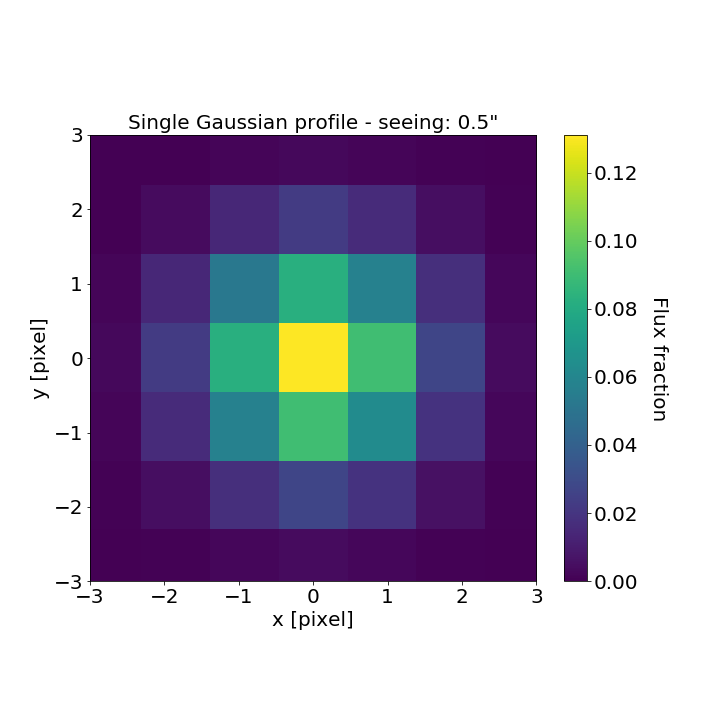
\includegraphics[width=0.6\textwidth]{flux_dist_seeing.png}}
  \subfigure[Fraction of flux of the central pixel as a function of the source position in this pixel.]{\label{fig:fluxposition}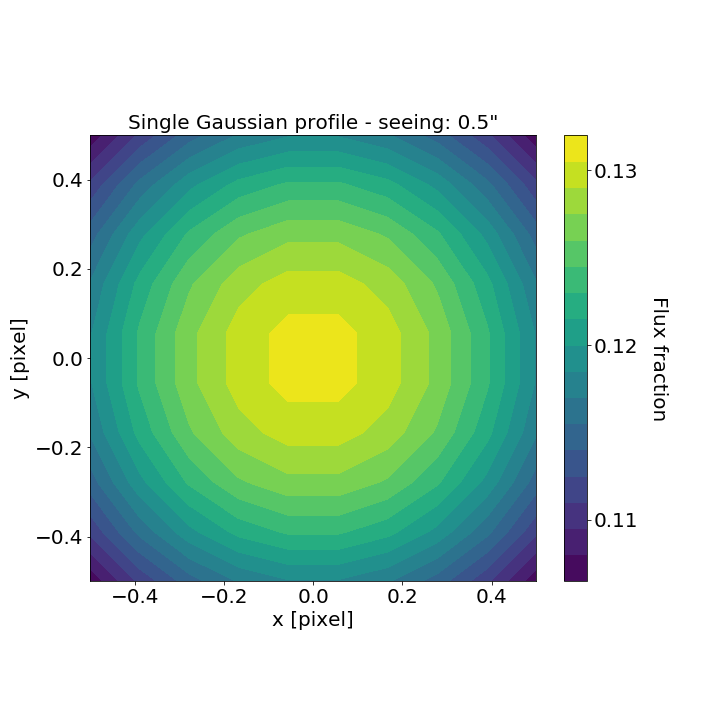
\includegraphics[width=0.6\textwidth]{flux_dist_center_position.png}}
  \caption{Flux distributions for a single gaussian PSF profile and a seeing of 0.5\arcsec.}\label{fig:fluxdist}
\end{figure}


A summary of the results obtained is given on Fig.\ref{fig:fracseeing} where the maximum fraction of flux in a pixel is displayed as a function of the seeing for a single gaussian (left) and a double gaussian (right) PSF profile. Highest fractions (typically 20 to 30\%) are reachable for seeing around 0.3\arcsec. The position of the source has a negligeable impact for seeings higher than 0.6\arcsec.
\begin{figure}[htbp]
\begin{center}
  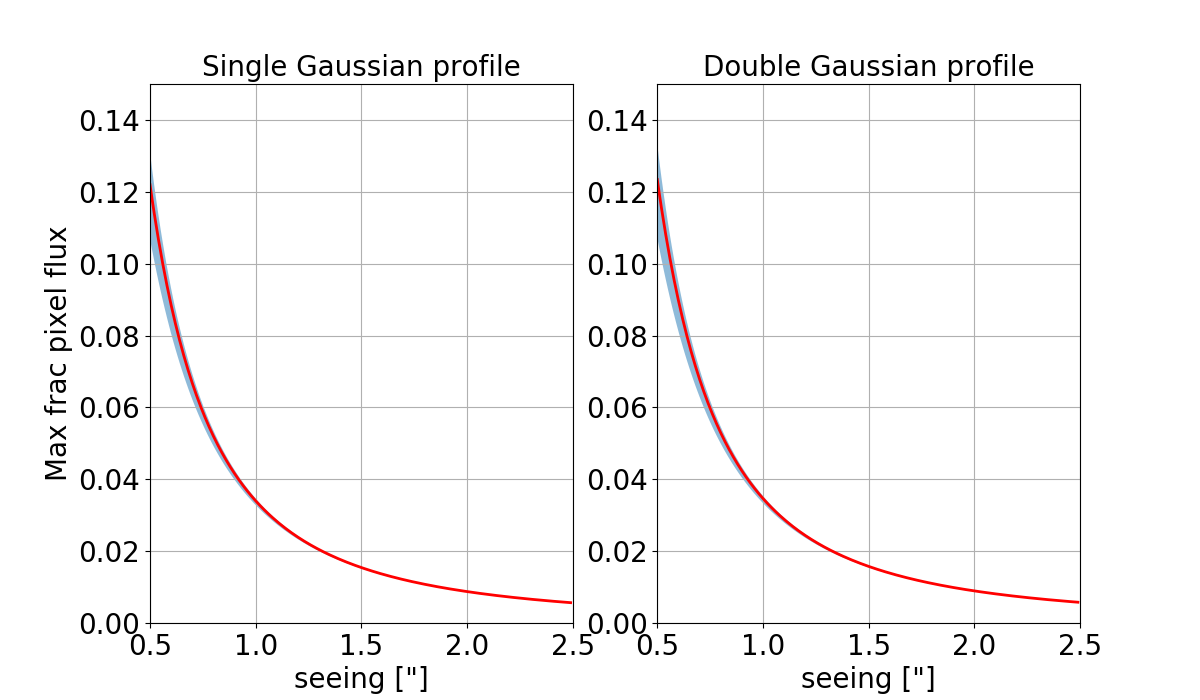
\includegraphics[width=0.9\textwidth]{max_frac_seeing.png}
 \caption{Maximum flux fraction (in a pixel) as a function of seeing for a single gaussian (left) and a double gaussian (right) PSF profile. The blue areas correspond to variations of the source position. Median values are represented by the red lines.}\label{fig:fracseeing}
\end{center}
\end{figure}

% ----------------------------------------------------------------------

\section{Saturation magnitude in LSST}
\label{sec:magsaturation}

It is possible to estimate the magnitude corresponding to pixel saturation by convolving  outcomes of Sect. \ref{sec:psfflux} with LSST intrument model. The method is the following: 

% ----------------------------------------------------------------------

\section{Impact of saturation on type Ia supernovae light curves}
\label{sec:discussion}
\subsection{Seeing distributions}

\subsection{Impact on Signal-to-Noise Ratio}

\subsection{Impact on $\sigma_C$}

% ----------------------------------------------------------------------

\section{Conclusion}
\label{sec:conclusion}



% ----------------------------------------------------------------------

\subsection*{Acknowledgments}

%%% Here is where you should add your specific acknowledgments, remembering that some standard thanks will be added via the \code{desc-tex/ack/*.tex} and \code{contributions.tex} files.

%This paper has undergone internal review in the LSST Dark Energy Science Collaboration. % REQUIRED if true


 % Standard papers only: author contribution statements. For examples, see http://blogs.nature.com/nautilus/2007/11/post_12.html

% This work used TBD kindly provided by Not-A-DESC Member and benefitted from comments by Another Non-DESC person.

% Standard papers only: A.B.C. acknowledges support from grant 1234 from ...

\input{desc-tex/ack/standard} % also available: key standard_short

% This work used some telescope which is operated/funded by some agency or consortium or foundation ...

% We acknowledge the use of An-External-Tool-like-NED-or-ADS.

%{\it Facilities:} \facility{LSST}

% Include both collaboration papers and external citations:
\bibliography{main,lsstdesc}

\end{document}

% ======================================================================
